\documentclass[17pt]{beamer}
\usepackage{graphicx}
\usepackage{tikz}
\usetikzlibrary{arrows,shapes,decorations,automata,backgrounds,petri,bending,positioning}
\usepackage{tikz-cd}
\usepackage{amsfonts}
\usepackage{amssymb}
\usepackage{amsmath}
\usepackage{amscd}
\usepackage{amsthm}
\usepackage{bbm}
\usepackage{fourier}
\usepackage[utf8]{inputenc}
\title{Wissenschaftslogik Erneuert}
\author{Hans Halvorson}
\date{June 6, 2018}
\setbeamertemplate{footline}{}
\setbeamertemplate{page number in head/foot}[totalframenumber]
\setbeamertemplate{navigation symbols}{\footnotesize\usebeamertemplate{page number in head/foot}}
\newcommand{\btVFill}{\vskip0pt plus 1filll}
%\setbeamertemplate{navigation symbols}{}%remove navigation symbols
\usepackage{eucal}
\setbeamercolor{normal text}{fg=black,bg=white}
\setbeamercolor{alerted text}{fg=red}
\setbeamercolor{example text}{fg=black}
\usepackage[absolute,overlay]{textpos}
\begin{document}
\def\2{\mathcal}
\def\7{\mathfrak}

\begin{frame}

\maketitle  %% the invariant content of equivalent theories

\end{frame}

\begin{frame}{\small introduction}

  A modest proposal for reinvigorating \newline
  -- logically rigorous \newline
  -- perspicuous \newline
  -- tractible \newline
  -- relevant \newline
  philosophy of science \newline

\end{frame}


\begin{frame}{precis of a forthcoming book}

  H. Halvorson, \emph{The Logic in Philosophy of Science}.  Cambridge
  University Press

  \bigskip Big thanks to Thomas Barrett and Neil Dewar

  \bigskip
  \url{www.princeton.edu/~hhalvors/main.pdf}


\end{frame}


\begin{frame}{\small biased historical overview}


\begin{itemize}
\item c 1900. the new logic
\item c 1935. Carnap's syntax program
\item c 1965. RIP syntax program
%% received view of theories
\end{itemize}

\end{frame}


\begin{frame}{\small biased historical overview}

\begin{itemize}
\item c 1975. the semantic view of theories
\item c 1995. RIP general philosophy of science
\item c 2009. philosophy of X proceeds on basis of semantic view
  %% Lagrangian-Hamiltonian, Belot and Baker on symmetry, wavefunction realism, Ramsey sentences

\end{itemize}


\end{frame}

\begin{frame}{\small Carnap's syntax program}

\begin{itemize}
\item Non-Euclidean geometry and de-interpretation (abstraction)
  %% pull a pattern off an instance that can be applied to other instances
  %% e.g. think of Z as an instance of the Group concept
  %% e.g. think of the Group concept as an instance of the Category concept

\item Philosophical stances clarified

  %% already in Aufbau, the two types of construction system are extensionally equivalent

\item What are \emph{syntactic} concepts?
  
\end{itemize}

\end{frame}

\begin{frame}{\small second semantic ascent}

\begin{enumerate}
\item What structure do theories have?
\item What structure does the universe of theories have?
\end{enumerate}

\end{frame}


\begin{frame}{\small category-theoretic analogy}

  \begin{tabular}{| l | l | l |}
    \hline 
material & formal & 2-formal \\ \hline \hline    
$\mathbb{Z}$ & $\mathbf{Grp}$ & $\mathbf{Cat}$ \\ \hline
  Hund & ``Hund'' &  word  \\ \hline
argument & modus ponens & valid forms \\ \hline \end{tabular}

\end{frame}

\begin{frame}{\small the universe of theories}

  \begin{figure}
    \centering
    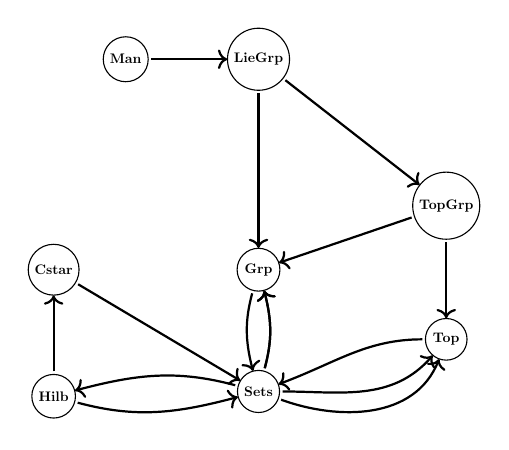
\begin{tikzpicture}
      \node [draw,circle,scale=0.5] (grp) {$\mathbf{Grp}$};
      \node [draw,circle,below= 1cm of grp,scale=0.5] (sets)
      {$\mathbf{Sets}$};
      \draw[thick,->,shorten <=1pt] (grp) to [out=255,in=105] (sets);
      \draw[thick,->,shorten <=1pt] (sets) to [out=75,in=285] (grp);
      \node [draw,circle,scale=0.5,below right=0.5cm and 2cm of grp]
      (top) {$\mathbf{Top}$};
      \draw[thick,->,shorten <=1pt] (sets) to [out=75,in=285] (grp);
      \node [draw,circle,scale=0.5,above=1cm of top] (topgrp)
      {$\mathbf{TopGrp}$};
      \draw[thick,->,shorten <=1pt] (topgrp) to (grp);
      \draw[thick,->,shorten <=1pt] (topgrp) to (top);
      \draw[thick,->,shorten <=1pt] (top) to [out=180,in=20](sets);
      \draw[thick,->,shorten <=1pt] (sets) to [out=0,in=230](top);
      \draw[thick,->,shorten <=1pt] (sets) to [out=-20,in=250] (top);
      \node [draw,circle,scale=0.5,above=2cm of grp] (liegrp)
      {$\mathbf{LieGrp}$};
      \node [draw,circle,scale=0.5,left=1cm of liegrp] (man)
      {$\mathbf{Man}$};
      \draw[thick,->,shorten <=1pt] (liegrp) to (grp);
      \draw[thick,->,shorten <=1pt] (man) to (liegrp);
      \draw[thick,->,shorten <=1pt] (liegrp) to (topgrp);
      \node [draw,circle,scale=0.5,left=2cm of grp] (cstar)
      {$\mathbf{Cstar}$};
      \node [draw,circle,scale=0.5,below=1cm of cstar] (hilb)
      {$\mathbf{Hilb}$};
      \draw[thick,->,shorten <=1pt] (cstar) to (sets);
      \draw[thick,->,shorten <=1pt] (hilb) to (cstar);
      \draw[thick,->,shorten <=1pt] (sets) to [out=165,in=15](hilb);
      \draw[thick,->,shorten <=1pt] (hilb) to [out=-15,in=195](sets);
      \end{tikzpicture}
    \end{figure}


\end{frame}

\begin{frame}{\small baby steps: propositional theories}

  Henkin algebra of $T$: equivalence classes of sentences under
  $T$-provable equivalence \newline
  
\bigskip
\begin{tabular}{| l | l |} \hline \hline
  $\mathbf{Th}$ & $\mathbf{Bool}$ \\ \hline 
  equivalence & isomorphism \\ \hline
  reduction & monomorphism  \\ \hline
  strengthening & epimorphism \\ \hline \end{tabular}

\end{frame}

\begin{frame}{\small realism and theoretical equivalence}

\begin{center}
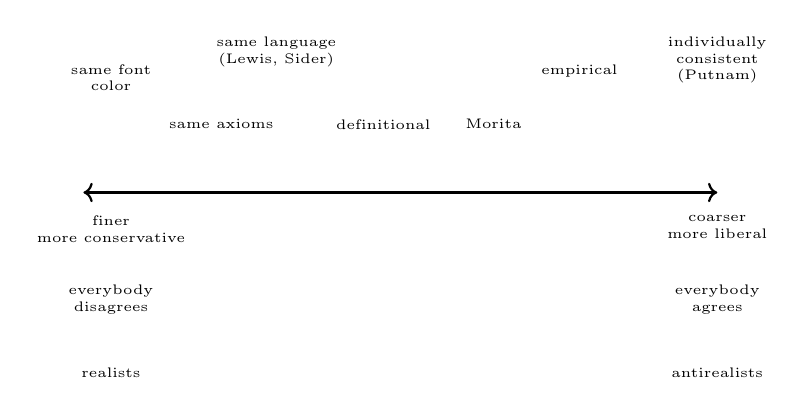
\begin{tikzpicture}[scale=0.7]
\tikzstyle{every node}=[font=\tiny]
\draw [<-> ,thick ] (-2.5,0) -- (9,0);
\node[align=center, below] at (-2,2.5) {same font \\ color};
\node[align=center, below] at (1,3) {same language \\ (Lewis, Sider)};
\node[align=center, below] at (0,1.5) {same axioms};
\node[align=center, below] at (3,1.5) {definitional };
\node[align=center, below] at (5,1.5) {Morita };
\node[align=center, below] at (6.5,2.5) {empirical};
\node[align=center, below] at (-2,-0.25) {finer \\ more conservative};
\node[align=center, below] at (9,-0.25) {coarser \\ more liberal};
\node[align=center, below] at (9,3) {individually \\ consistent \\ (Putnam)};
\node[align=center, below] at (-2,-1.5) {everybody  \\ disagrees};
\node[align=center, below] at (-2,-3) {realists};
\node[align=center, below] at (9,-1.5) {everybody \\ agrees};
\node[align=center, below] at (9,-3) {antirealists};
\end{tikzpicture}
\end{center}  
\end{frame}

\begin{frame}{\small Hamiltonian and Lagrangian mechanics}

  \begin{itemize}
\item North (2009): H and L cannot be equivalent because their models are
  not isomorphic
\item Model Isomorphism Criterion of Theoretical Equivalence: $T$ and
  $T'$ are equivalent only if each model $M$ of $T$ is isomorphic to a
  model $M'$ of $T'$.
\end{itemize}

\end{frame}

\begin{frame}{\small believing a scientific theory}

  \begin{itemize}
  \item Semantic Account of Belief (van Fraassen, Giere): to accept
    $T$ means to believe that one of its models $M$ is isomorphic to
    the world.
  \item Stipulation: If $T$ and $T'$ are equivalent, then any reason
    to accept $T$ is a reason to accept $T'$.
  \item Corollary: If $\neg$MIC then $\neg$SB
    \end{itemize}

  \end{frame}


\begin{frame}[fragile]{\small Ramsey equivalence (Dewar)}

  \begin{figure}
    \begin{tikzcd}
      & T_1^R \equiv T_2^R & \\
      T_1 \arrow{ur} & & T_2 \arrow{ul} \end{tikzcd} \end{figure}

  
Full semantics: Empirical-E $\Leftrightarrow$ Ramsey-E

Frame semantics: Definitional-E $\not\Rightarrow$ Ramsey-E


\end{frame}
  

\begin{frame}{\small wavefunction realism}

  \begin{quote} The wave function simply represents reality
    directly. (Sean Carroll) \end{quote}

  \begin{quote} The quantum state is a mere calculation device. (Carlo
    Rovelli) \end{quote}
    


\end{frame}
  

\begin{frame}{\small flat vs.\ structured views of theories}

  \begin{tabular}{r | c | c |}
    & flat  & structured \\ \hline
    syntactic & Quine        & \\ \hline
    semantic  & van Fraassen & \\ \hline
  \end{tabular}

  \bigskip Claim: Flat views of theories entail immoderate views of
  theoretical equivalence.


\end{frame}


\begin{frame}{\small varieties of symmetry}

  \begin{figure}
    \centering
  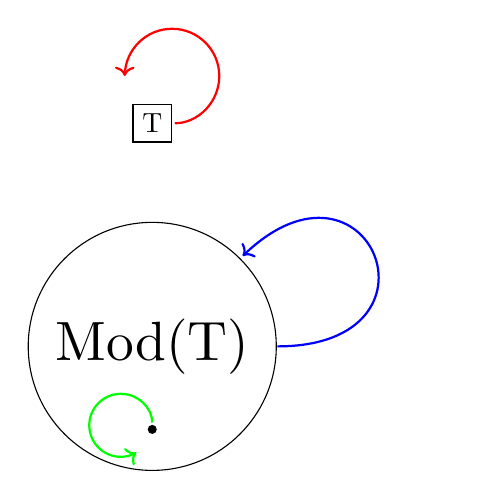
\begin{tikzpicture}
    \node [draw] (a) {T};
    \draw[red,thick,->,shorten <=1pt] (a.0) arc (-90:180:6mm);
    \node[draw,circle,scale=2] (b) [below= 1cm of a] {Mod(T)};
    \draw[blue,thick,->,shorten >=1pt] (b) to [out=0,in=45,loop,looseness=4.8] (b);
    % \draw[blue,thick,->,shorten <=1pt,shorten >=20pt] (b.-25) arc (-75:180:20mm);
    \node[circle,draw,fill=black,scale=0.3] (c) at
    ([yshift=-3em]b.center){};
 \draw[green,thick,->,shorten <=1pt] (c.90) arc (0:300:4mm);   
  \end{tikzpicture}  
\end{figure}

\end{frame}


\begin{frame}{\small counting possibilities}

  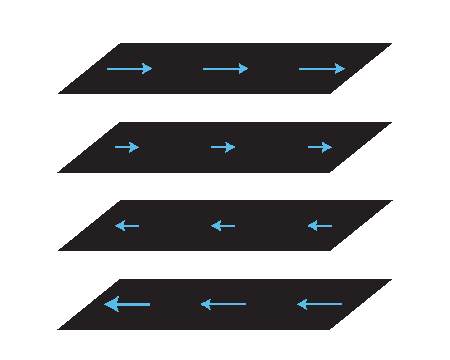
\includegraphics[scale=1]{galileanboost.pdf}

  Does a shift generate a new possibility? 

\end{frame}


\begin{frame}{\small counting possibilities}

\begin{description}
\item[shiftless] isomorphic models represent same possibility
  (Saunders, Baker)
\item[shifty] distinct models represent distinct possibilities
  (Belot) \end{description}

\end{frame}

\begin{frame}[fragile]{\small category of models}
  \begin{figure}
    \centering  
  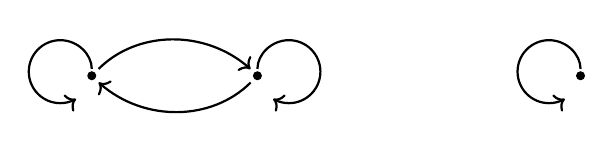
\begin{tikzpicture}
    \node [circle,draw,fill=black,scale=0.3] (a) {};
    \draw[thick,->,shorten <=1pt] (a.90) arc (0:300:4mm);
    \node[circle,draw,fill=black,scale=0.3] (b) [right= 2cm of a]
    {};
    \draw[thick,->,shorten <=1pt] (b.90) arc (180:-120:4mm);
    \draw[thick,->,shorten >=2pt,shorten <=2pt] (a) to [out=45,in=135] (b);
    \draw[thick,->,shorten >=2pt,shorten <=2pt] (b) to
    [out=-135,in=-45] (a);
    \node[circle,draw,fill=black,scale=0.3] (c) [right= 4cm of b]
    {};
    \draw[thick,->,shorten <=1pt] (c.90) arc (0:300:4mm);
  \end{tikzpicture}
\end{figure}

Models are objects in a category (and nothing more) $\Longrightarrow$
possibilities cannot be counted
  
\end{frame}



\begin{frame}{\small ethics of Wissenschaftslogik}

  \begin{itemize}
  \item Hegel: after all analyses are complete, no remaining freedom
    of choice  
  \item Carnap: in logic there are no morals
  \item Quine: no place for value judgments
  \item Carnap$^+$: logic in the service of morals
 \end{itemize}   
    
\end{frame}

    



\end{document}




%% NB Religion Analogy


\begin{frame}{\small radical right wing}


\begin{center}
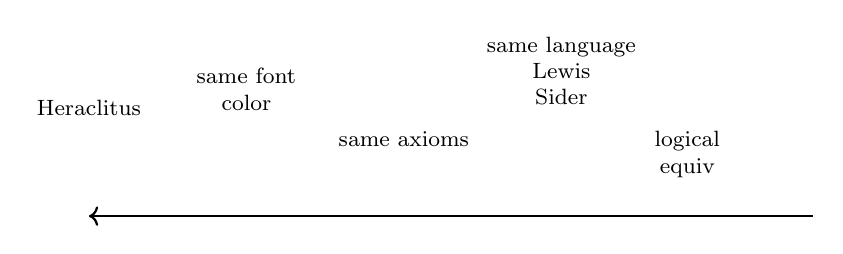
\begin{tikzpicture}[scale=0.8]
\tikzstyle{every node}=[font=\footnotesize]
\draw [<- ,thick ] (-3.5,0) -- (8,0);
\node[align=center, below] at (-3.5,2) {Heraclitus};
\node[align=center, below] at (-1,2.5) {same font \\ color};
\node[align=center, below] at (4,3) {same language \\ Lewis \\ Sider};
\node[align=center, below] at (1.5,1.5) {same axioms};
\node[align=center, below] at (6,1.5) {logical \\ equiv};

\end{tikzpicture}
\end{center}





%% same language -- logical equivalence -- same axioms -- same font -- token theory

%% protestants fighting over baptism -- only my beliefs are correct

%% (ideological purity)


\end{frame}



\begin{frame}{\small radical left wing}

%% structuralism -- Goodmania


%% all religions are the same -- everyone believes in God (or not)

\begin{center}
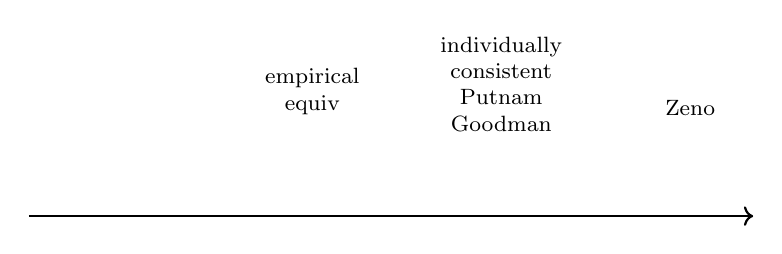
\begin{tikzpicture}[scale=0.8]
\tikzstyle{every node}=[font=\footnotesize]
\draw [-> ,thick ] (-1.5,0) -- (10,0);
\node[align=center, below] at (3,2.5) {empirical \\ equiv};
\node[align=center, below] at (6,3) {individually \\ consistent \\
  Putnam \\ Goodman};
\node[align=center, below] at (9,2) {Zeno};
\end{tikzpicture}
\end{center}




\end{frame}


\begin{frame}{\small the ideological spectrum}

\begin{center}
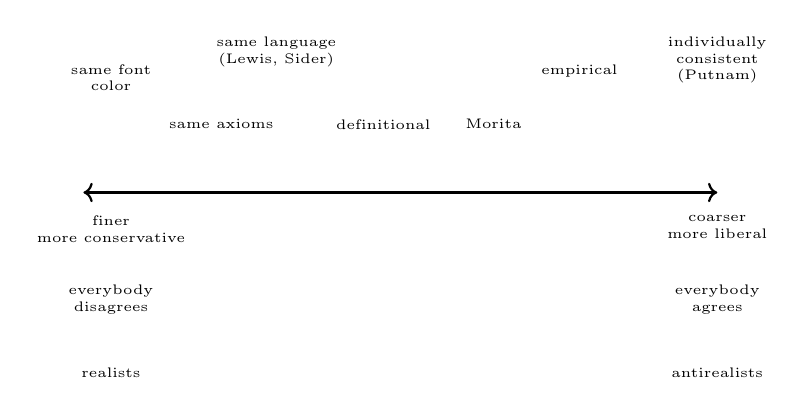
\begin{tikzpicture}[scale=0.7]
\tikzstyle{every node}=[font=\tiny]
\draw [<-> ,thick ] (-2.5,0) -- (9,0);
\node[align=center, below] at (-2,2.5) {same font \\ color};
\node[align=center, below] at (1,3) {same language \\ (Lewis, Sider)};
\node[align=center, below] at (0,1.5) {same axioms};
\node[align=center, below] at (3,1.5) {definitional };
\node[align=center, below] at (5,1.5) {Morita };
\node[align=center, below] at (6.5,2.5) {empirical};
\node[align=center, below] at (-2,-0.25) {finer \\ more conservative};
\node[align=center, below] at (9,-0.25) {coarser \\ more liberal};
\node[align=center, below] at (9,3) {individually \\ consistent \\ (Putnam)};
\node[align=center, below] at (-2,-1.5) {everybody  \\ disagrees};
\node[align=center, below] at (-2,-3) {realists};
\node[align=center, below] at (9,-1.5) {everybody \\ agrees};
\node[align=center, below] at (9,-3) {antirealists};
\end{tikzpicture}
\end{center}




\end{frame}



\begin{frame}{non-absurd views}



\begin{center}
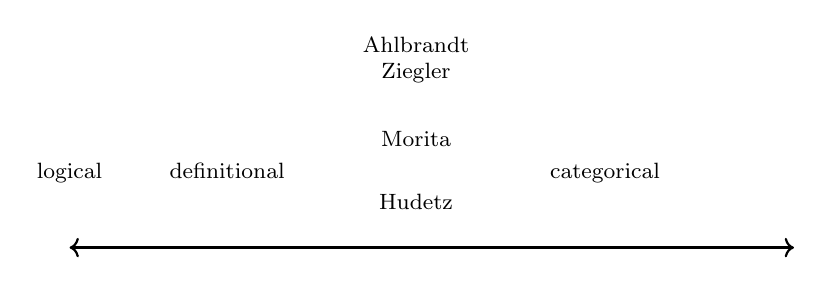
\begin{tikzpicture}[scale=0.8]
\tikzstyle{every node}=[font=\footnotesize]
\draw [<-> ,thick ] (-1.5,0) -- (10,0);
\node[align=center, below] at (-1.5,1.5) {logical};
\node[align=center, below] at (1,1.5) {definitional};
\node[align=center, below] at (4,2) {Morita};
\node[align=center, below] at (4,1) {Hudetz};
\node[align=center, below] at (4,3.5) {Ahlbrandt \\ Ziegler};
\node[align=center, below] at (7,1.5) {categorical};
\end{tikzpicture}
\end{center}


%% my goal: push you into left wing of sanity zone

\end{frame}




\begin{frame}{\small logical equivalence}

\begin{itemize}
\item $T_1$ and $T_2$ are \textbf{logically equivalent} just in case
they are in the \textbf{same} signature and:
\[ \mathrm{Cn}(T_1)=\mathrm{Cn}(T_2) \]
\[ \mathrm{Mod}(T_1)=\mathrm{Mod}(T_2) \]
\item Overly restrictive: same signature
\end{itemize}


\end{frame}



\begin{frame}{\small definitional extension}

\begin{itemize}
\item Example: define $\leq$ by 
\[ \forall x,y(x\leq y\leftrightarrow (x<y\vee x=y)) \]
\item \textbf{Defn:} $T^+$ is a \textbf{definitional extension} of $T$
  just in case for each new relation symbol $r$ of $\Sigma ^+$, there
  is a formula $Fr$ of $\Sigma$ such that:
\[ T^+ \: \vdash \: \forall \overline{x}(r(\overline{x})\leftrightarrow (Fr)(\overline{x})) .\]
\end{itemize}


\end{frame}



\begin{frame}{\small definitional extension}

\begin{itemize}
\item $r\mapsto Fr$ extends to an \textbf{interpretation} $F:T^+\to
  T$.
\item Each model $M$ of $T$ is uniquely expandable to a model $F^*(M)$
  of $T^+$, where
  \[ M\vDash (F\phi)(\overline{a}) \quad \Longleftrightarrow \quad
  F^*(M)\vDash \phi (\overline{a}) \]
\end{itemize}

\end{frame}


\begin{frame}

  {\small $T_1$ and $T_2$ are \textbf{definitionally equivalent} if they have
  a \textbf{common definitional extension}.}

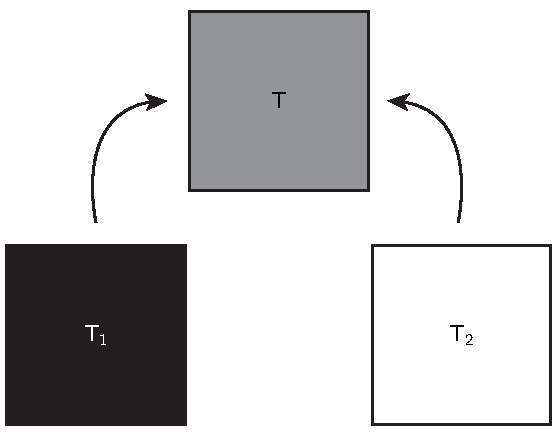
\includegraphics{definitionalequivalence.pdf}

\end{frame}


\begin{frame}{\small definitional equivalence}

  \textbf{Prop:} $T_1$ and $T_2$ are definitionally equivalent if and
  only if there are \textbf{direct} translations $F:T_1\to T_2$ and
  $G:T_2\to T_1$ that are quasi-inverse to each other.


\end{frame}


\begin{frame}{\small invariants of DEF}

\begin{enumerate}
\item numerical claims
\item cardinality of models
\item definable subsets of models
\end{enumerate}


\end{frame}


\begin{frame}{\small reasons to liberalize}

\begin{itemize}

\item Direct translation is overly restrictive 

%   e.g.\ the reduction of $\mathbb{C}$ to $\mathbb{R}$ is not a direct
%  translation

\item DEF too restrictive for the scientific \& mathematical
  mainstream

\begin{itemize}

\item Wave vs Matrix mechanics

\item Tarski's axiomatizations of geometry

\item Dualities in math and physics 

\end{itemize}


\end{itemize}



%% still an attachment to a common linguistic element -- base sort

%% scientific practice

%%  - geometry

%%  - Schrodinger and Heisenberg

%%  - dualities


\end{frame}


\begin{frame}{\small categorical equivalence}

Consider $\mathrm{Mod}(T)$ as consisting of two kinds of things:

\begin{description}
\item[objects] models of $T$
\item[arrows] elementary embeddings of models
\end{description}


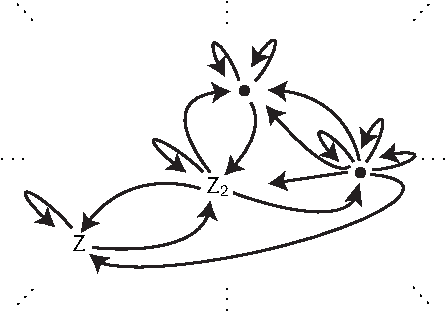
\includegraphics{grp1category.pdf}

%% to do: explain category of models

%% relations between models - embedding, symmetry, cover

%% *functor* takes models to models [but no restriction!], arrows to
%% arrows of the same type

%% $F$ is an equivalence -- two notions


\end{frame}

\def\3{\mathbf}


\begin{frame}{\small categorical equivalence}

objects of $\3C$  $\quad \longmapsto \quad$ objects of $\3D$ 

\bigskip arrows of $\3C$ $\quad \longmapsto \quad$ arrows of $\3D$

\bigskip (1) plays nicely with composition of arrows \\
(2) quasi-invertible 




\end{frame}

\begin{frame}

  \begin{center} logical $\:\Longrightarrow\:$ definitional
      $\:\Longrightarrow\:$ categorical 
\end{center}


\end{frame}



\begin{frame}{\small Goodmania?}

\begin{tabular}{l  l}

  $T_1$ & There is exactly one thing, \\ & named $c_1$. \\ \\ 
  $T_{17}$ & There are exactly seventeen things, \\ 
& named $c_1,c_2,\dots
  ,c_{17}$ \end{tabular}

\vspace{2em} \begin{center} \textcolor{red}{\danger} \quad $\mathrm{Mod}(T_1)\:\equiv\:
\mathrm{Mod}(T_{17})$ \quad \textcolor{red}{\danger} \end{center}

  %% Do categorically equivalent theories *say* the same thing about
  %% the world?

%% "there is just one named thing," versus "there are seventeen named things"?

  %% could quantum mechanics be categorically equivalent to general
  %% relativity??

\end{frame}

%% finding the sweet spot somewhere around definitional equivalence
%% and categorical equivalence


\begin{frame}{\small Morita equivalence}

\begin{itemize}
\item \textbf{many-sorted logic:} Signatures include \textbf{sort
    symbols}, rather than just relation symbols.
\item Morita extension:
\begin{itemize}
\item product sorts
\item quotient sorts
\item subsorts
\item coproduct sorts
\end{itemize}
\item \textbf{Defn:} $T_1$ and $T_2$ are \textbf{Morita equivalent}
  just in case they have a common Morita extension.
\end{itemize}




\end{frame}

\begin{frame}{\small Morita equivalence}

  Morita $\:\Longrightarrow \:$ categorical

\bigskip Invariant lost: cardinality of models

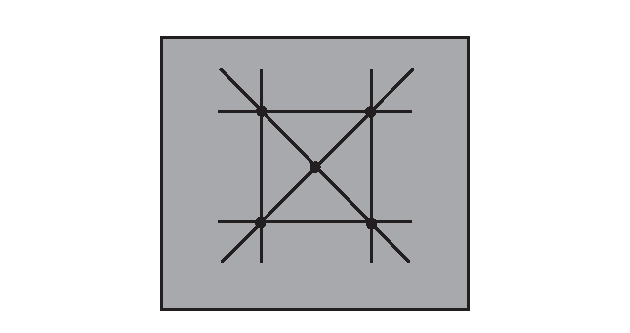
\includegraphics{affine1.pdf}

\end{frame}



\begin{frame}

\begin{center} {\small logical $\:\Longrightarrow\:$ definitional $\:\Longrightarrow\:$
Morita $\:\Longrightarrow\:$ categorical }  \end{center}

\end{frame}


\begin{frame}{\small Ahlbrandt-Ziegler equivalence}

\begin{itemize}
\item \textbf{Defn:} An $m$-dimensional \textbf{translation} $F:T_1\to
  T_2$ assigns to each formula $\phi (\overline{x})$ of $T_1$, a
  formula $(F\phi )(\overline{y}_1,\dots ,\overline{y}_m)$ of $T_2$.
\item \textbf{Fact:} A translation $F:T_1\to T_2$ induces a functor
  $F^*:\mathrm{Mod}(T_2)\to \mathrm{Mod}(T_1)$.
\end{itemize}
\end{frame}

\begin{frame}{\small AZ equivalence}

  \textbf{Defn:} $T_1$ and $T_2$ are \textbf{AZ equivalent} just in
  case there is a translation $F:T_1\to T_2$ such that
  $F^*:\mathrm{Mod}(T_2)\to \mathrm{Mod}(T_1)$ is an equivalence of
  categories. 


\end{frame}


\begin{frame}

\begin{center} {\small logical $\:\Longrightarrow\:$ definitional $\:\Longrightarrow\:$
AZ $\:\Longrightarrow\:$ categorical}  \end{center}

\end{frame}



\begin{frame}{\small conjecture}

  \begin{center} {\LARGE Morita
      $\quad\stackrel{?}{\Longleftrightarrow}\quad$ AZ} \end{center}


\end{frame}


\begin{frame}{\small application: Hamiltonian and Lagrangian mechanics}


\begin{itemize}
\item J. North: ``Hamiltonian and Lagrangian mechanics are not
  equivalent in terms of statespace structure.  This means that they
  are not equivalent, period.''
\item T. Barrett: Hamiltonian and Lagrangian mechanics are
  categorically equivalent.
\end{itemize}


\end{frame}


\begin{frame}{\small application: acceptance}


\begin{itemize}
\item ACCEPT: To accept $T$ is to believe that one of the models of
  $T$ is isomorphic to WORLD.
\item EQUIV: If $T_1$ is equivalent to $T_2$, then to accept $T_1$ is
  to accept $T_2$.
\item Morita + EQUIV rules out ACCEPT.
\end{itemize}


\end{frame}


\begin{frame}{\small application: wavefunction realism}

\begin{itemize}
\item $\mathbf{Hilb}$ is categorically equivalent to $\mathbf{CStar}$
\item $\mathbf{CStar}$ doesn't talk about wavefunctions.
\item So, take your wavefunction \emph{cum grano salis}. \end{itemize}

\end{frame}


\begin{frame}{\small conclusions}

\begin{itemize}
\item Carnapian tolerance: there is no question of \emph{correctness}
  when it comes to notions of theoretical equivalence.
\item Second order morals: (1) clarity, \newline (2) tolerance of
  dissenters.
\end{itemize}

\end{frame}





\end{document}










\begin{frame}{The resemblance view of representation}




\end{frame}


\begin{frame}{A cardinal error in the semantics of science}

  ``A theory is true only if one of its models is isomorphic to
  WORLD.''

\end{frame}

\begin{frame}

\begin{enumerate}


\item Two theories are equivalent only if their models are isomorphic.

\end{enumerate}



\end{frame}


\begin{frame}{The model isomorphism criterion for theoretical
    equivalence (MIC)}

\begin{exampleblock}{}
  $T$ and $T'$ are equivalent only if their models are isomorphic.
\end{exampleblock}

\end{frame}

\begin{frame}



\end{frame}

\begin{frame}{The trouble with IC}

  The notion of isomorphism is relative to a species of mathematical
  structure.


\end{frame}

\end{document}

\begin{frame}{Example}

\begin{itemize}
\item Linear orderings in signature $\{ < \}$.
\item Linear orderings in signature $\{ \leq \}$. 
\end{itemize}


\end{frame}

\begin{frame}{Example}


\begin{center}
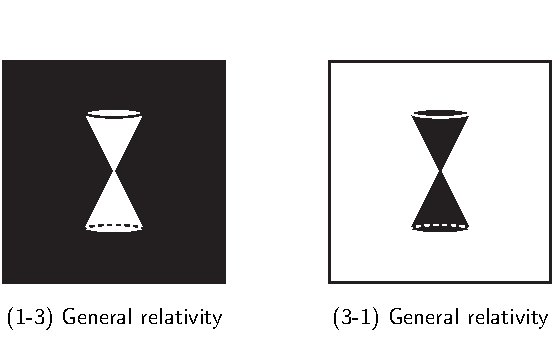
\includegraphics{1-3v3-1.pdf}
\end{center}


\end{frame}

\begin{frame}{The isomorphism theory of truth (ITT)}

  \begin{exampleblock}{} A theory is \textbf{true} if the real world
    itself is isomorphic to one of the theory's models.
\end{exampleblock}


\end{frame}


\begin{frame}{The trouble for ITT}

ITT $\Longrightarrow$ IC

\end{frame}

\begin{frame}{The hunt for artifact-free representations}

\begin{enumerate}
\item Example: coordinate free geometric theories 
\item Example: comparativism about quantity 
\end{enumerate}

\end{frame}



\begin{frame}

  A \textbf{signature} $\Sigma$ is a set of sort symbols, relation
  symbols, function symbols, and constant symbols.

\bigskip 

$\Sigma =\{ s_1,s_2,p,q \}$


\end{frame}


\begin{frame}

 \begin{center}
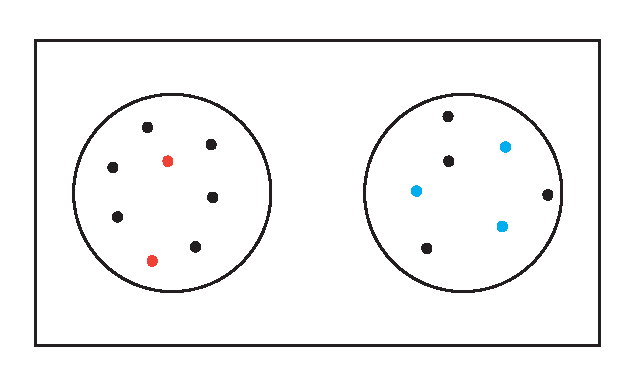
\includegraphics{sigmastructure.pdf}

A $\Sigma$-structure
\end{center}

  

\end{frame}


\begin{frame}

\begin{itemize}
\item there is a unique $x$ of sort $s_1$ that is $p$.
\item there is a unique $y$ sort $s_2$ that is $q$.
\end{itemize}

\bigskip
A $\Sigma$-theory $T$

\end{frame}

\begin{frame}

 \begin{center}
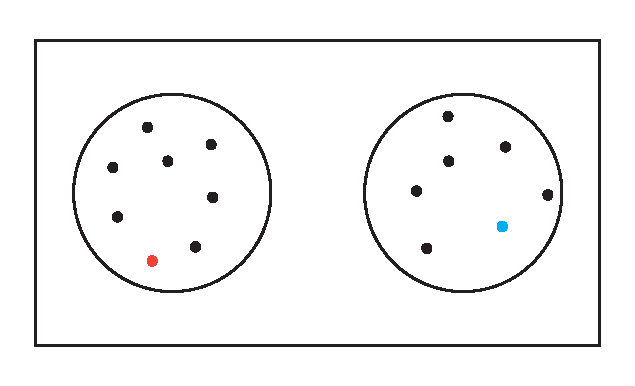
\includegraphics{Tmodel.pdf}

A model of the $\Sigma$-theory $T$
\end{center}


\end{frame}

\begin{frame}

Two theories are \textbf{logically equivalent} if they have the same
class of models. \end{frame}

\begin{frame}

\begin{itemize}
\item there is a unique $x$ of sort $s_1$ that is $p$ and there is a
  unique $y$ of sort $s_2$ that is $q$.
\end{itemize}

\bigskip
A theory $T'$ that is logically equivalent to $T$


\end{frame}


\begin{frame}

There are many pairs of theories that are not logically equivalent,
but are nonetheless intuitively equivalent.  

\end{frame}


\begin{frame}

\begin{itemize}
\item Linear orderings in signature $\{ \leq \}$.
\item Linear orderings in signature $\{ < \}$.
\end{itemize}

\end{frame}


\begin{frame}
\begin{itemize}
\item The theory that says, ``there is a $p$'', in the signature $\{ p
  \}$.
\item The theory that says, ``there is a $q$'', in the signature $\{ q
  \}$.
\end{itemize}

\end{frame}

\begin{frame}

A \textbf{definitional extension} of a theory $T$ is a theory $T^+$
obtained by adding to $T$ definitions of new predicate symbols,
function symbols, and constant symbols. 

\end{frame}


\begin{frame}

Example: ZFC formalized in $\{ \in \}$.  Define a relation $\subseteq$
by 
$$ (x\subseteq y )\: \leftrightarrow \: \forall z(z\in x\to z\in y) .$$


\end{frame}


\begin{frame}

Two theories are \textbf{definitionally equivalent} if they have a
common definitional extension. \end{frame}


\begin{frame} There are pairs of theories that are not definitionally
  equivalent, but are nonetheless intuitively equivalent. \end{frame}

\begin{frame}

\begin{itemize}
\item The empty theory in signature $\{ s_1,s_2\}$.
\item The theory in signature $\{ s,p,q\}$ that says there is an $x$
  that is $p$, a $y$ that is $q$, and every $z$ is either $p$ or $q$
  but not both.
\end{itemize}

\end{frame}


\begin{frame}

 \begin{center}
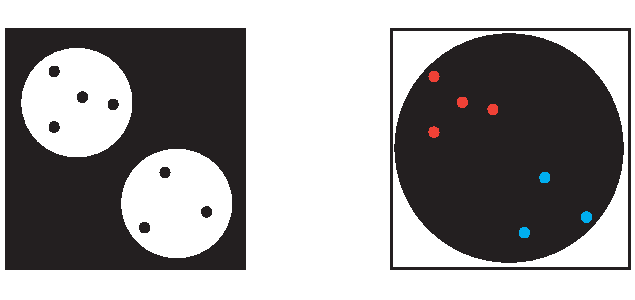
\includegraphics{quineexamplemodels.pdf}

models of these two theories
\end{center}

\end{frame}

\begin{frame}

A \textbf{Morita extension} of a theory $T$ is a theory $T^+$ obtained
by adding to $T$ definitions of new sort symbols, relation symbols,
function symbols, and constant symbols. 

\end{frame}

\begin{frame}

Two theories are \textbf{Morita equivalent} if they have a common
Morita extension. 

\end{frame}

\begin{frame}{Realism without naivete}

\begin{itemize}
\item $\Sigma = \{ s\}$.  $T$ says that there are exactly two things.
\item $\Sigma = \{ s_1,s_2 \}$.  $T'$ says that there are two things
  of type $s_1$, and four things of type $s_2$.  Things of type $s_2$
  are ordered pairs of things of type $s_1$.
\end{itemize}


\end{frame}



\begin{frame}

  \emph{Unfortunately}, Morita equivalence doesn't generalize directly
  to theories beyond the ambit of first-order logic.  \end{frame}

\begin{frame}

\begin{itemize}
\item First order theories have categories of models.
\item Physical theories have categories of models too. 
\end{itemize}

\end{frame}

\begin{frame}

\begin{center}
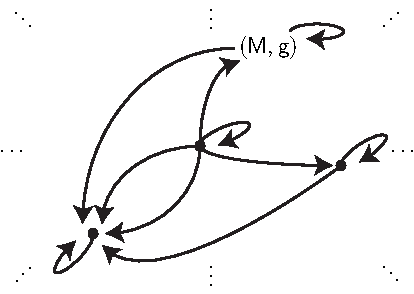
\includegraphics{grcategory.pdf}

The category of models for general relativity
\end{center}

\end{frame}


\begin{frame}

  Two theories are \textbf{categorically equivalent} if they have
  equivalent (structurally identical) categories of
  models. \end{frame}


\begin{frame}

\textbf{Theorem 1.} If two theories are Morita equivalent, then they
are categorically equivalent. \end{frame}


\begin{frame}

  \textbf{Theorem 2.} There are categorically equivalent theories that
  are not Morita equivalent. \end{frame}


\begin{frame}{The disappearance of structure?}

\begin{center}
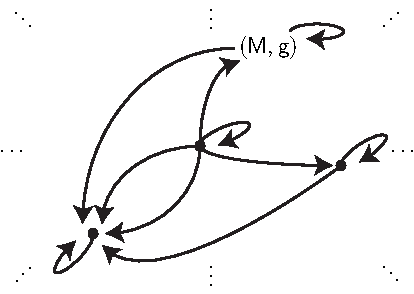
\includegraphics{grcategory.pdf}

The category of models for general relativity
\end{center}

\end{frame}



\end{document}

%%% Local Variables:
%%% mode: latex
%%% TeX-master: t
%%% End: